\documentclass[10pt,a4paper]{article}
\usepackage[utf8]{inputenc}
\usepackage[spanish]{babel}
\usepackage{amsmath}
\usepackage{amsfonts}
\usepackage{amssymb}
\usepackage{graphicx}
\usepackage{enumitem}
\usepackage{listings}

\usepackage[left=2cm,right=2cm,top=2cm,bottom=2cm]{geometry}




\begin{document}

\author{José Espinoza Peralta}
\title{Metodo de Newton para Sistemas de 2 ecuaciones no lineales}
\date{\small{\today}}
\maketitle

\tableofcontents

\newpage
\section{El método de Newton- Función variable real}
Método que se utiliza para calcular los ceros de una función real de variable real. Aunque no sea siempre el mejor método para un problema dado, su simplicidad formal y su rapidez de convergencia hacen que, con frecuencia, sea el primer algoritmo a considerar para esta tarea.

El método de Newton-Raphson se basa en el desarrollo de Taylor de la función cuya raíz se quiere calcular. Consideremos la ecuación $\boldsymbol{f(x)}=0$, y supongamos que posee una y sólo una solución $\alpha \in [a,b]$. Partiendo de un punto x0 suficientemente cercano a dicha raíz, podemos escribir: 
 
$$\boldsymbol{f(\alpha)=f(x_{0})+(\alpha-x_{0})f'(x_{0})+\frac{(\alpha-x_{0})^{2}}{2}f''(x_{0})+...}$$

Suponiendo que $f'(x)$ no se anula en $[a,b]$, y que la diferencia $\alpha-x_{0}$ es muy pequeñas, el método de Newton-Raphson consiste en despreciar los términos desde el sumando $(\alpha-x_{0})^{2}$ del desarrollo anterior, quedándonos con la aproximación: 

$$\boldsymbol{f(\alpha)\cong f(x_{0})+(\alpha-x_{0})f'(x_{0})}$$

Como $\alpha$ es la solución de la ecuación $\boldsymbol{f(x)}=0$ se tiene que $\boldsymbol{f(\alpha)}=0$ y por tanto, de la expresión anterior se sigue que: 
$$\boldsymbol{f(x_{0})+(\alpha-x_{0})f'(x_{0})\cong 0}$$

y despejando $\alpha$ resulta: 
$$\boldsymbol{\alpha \cong x_{0} -\frac{f(x_{0})}{f'(x_{0})}= x_{1}}$$

Así pues, si se parte de un valor $x_{0}$ próximo a $\alpha$, el valor siguiente $x_{1}$ obtenido de esta forma proporciona un valor más próximo a la raíz $\alpha$.
El proceso puede seguir repitiéndose sucesivamente hasta encontrar un $x_{k}$ lo suficientemente próximo a la raíz $\alpha$.

\section{Sistemas de ecuaciones no lineales}
Sea $\boldsymbol{f}:\mathbb{R}^{n}\rightarrow \mathbb{R}^{n}$ una función de varias variables, no-lineal. Se quiere resolver el sistema de ecuaciones $\boldsymbol{f(x)}=0$, donde $\boldsymbol{x}=(x_{1},...,x_{n})^{t} \in \mathbb{R}^{n}$ representa al vector de incógnitas. 

\section{El método de Newton- Función varias variables}
Una de las ventajas del método de Newton-Raphson ademas de su velocidad de convergencia, es que se puede generalizar fácilmente a sistemas de ecuaciones no lineales.\\

Supongamos que $\alpha=(\alpha_{1},...,\alpha_{n})^{t}\in \mathbb{R}^{n}$ es la solución del sistema de ecuaciones, y que $\boldsymbol{f}=(f_{1},...,f_{n})^{t}$ es dos veces diferenciable. Entonces aplicando el desarrollo de Taylor para funciones de varias variables de $\boldsymbol{f}$ en torno a una aproximación de la raíz $x^{(k)}=(x_{1}^{(k)},...,x_{n}^{(k)})^{t}$, se tiene que: 
 
$$\boldsymbol{0=f(\alpha)=f(x^{(k)})+J(x^{(k)})(\alpha-x^{(k)})+\mathcal{O}(\left \| \alpha-x^{(k)} \right \|^{2})}$$

Donde $J(x^{(k)})$ es la  \textbf{matriz Jacobiana} en $x^{(k)}:$. 

$$J(x^{(k)})=\begin{pmatrix}
\frac{\partial f_{1}}{\partial x_{1}}(x^{(k)}) & \cdots  & \frac{\partial f_{1}}{\partial x_{n}}(x^{(k)}) \\ 
\vdots  &  & \vdots  \\ 
\frac{\partial f_{n}}{\partial x_{1}}(x^{(k)}) & \cdots & \frac{\partial f_{n}}{\partial x_{n}}(x^{(k)})
\end{pmatrix}$$

Notamos que cuando $\left \| \alpha-x^{(k)} \right \|$ es pequeño, el término $\mathcal{O}(\left \| \alpha-x^{(k)} \right \|^{2})$ es mucho más pequeño aún y puede despreciarse en el desarrollo de Taylor anterior: 

$$\boldsymbol{0=f(x^{(k)})+J(x^{(k)})(\alpha-x^{(k)})+\mathcal{O}(\left \| \alpha-x^{(k)} \right \|^{2})}$$

$$\boldsymbol{\approx f(x^{(k)})+J(x^{(k)})(\alpha-x^{(k)})}$$

Si además la matriz $J(x^{(k)})$ es invertible, entonces podemos aproximar la raíz $alpha$ despejandola en la ecuación anterior: 
  $$\boldsymbol{\alpha \approx x^{(k)}-[J(x^{(k)})]^{-1}f(x^{(k)})}$$
  
El \textbf{método de Newton} consiste en, dada la aproximación de la solución $x^{(k)}$, tomar como nueva aproximación $x^{(k+1)}$ el valor de la expresión anterior:  

$$\boldsymbol{x^{(k+1)}:=x^{(k)}-[J(x^{(k)})]^{-1}f(x^{(k)})},\hspace{1cm} k=0,1,2,...$$

donde $x^{(0)}$ es la aproximación inicial. 


\section{El método de Newton- Sistema 2 ecuaciones}

Sea $\boldsymbol{f}:\mathbb{R}^{2}\rightarrow \mathbb{R}^{2}$ una función de 2 variables, no-lineal. Para el trabajo requerido, se quiere resolver el sistema de ecuaciones $\boldsymbol{f(x,y)}=(0,0)^{t}$. \\

Teniendo que $f(x,y)=(f_{1},f_{2})^{t}$ y su respectivo Jacobiano sea: 
$$J=\begin{pmatrix}
 \frac{\partial f_{1}}{\partial x} & \frac{\partial f_{1}}{\partial y}\\ 
 \frac{\partial f_{2}}{\partial x} & \frac{\partial f_{2}}{\partial y} 
\end{pmatrix}
$$



Por el metodo de Newton desarrollado anteriormente, tendremos que: 
$$\begin{pmatrix} x \\ y \end{pmatrix}^{k+1} = \begin{pmatrix} x \\ y \end{pmatrix}^{k}-J^{-1}\begin{pmatrix} x \\ y \end{pmatrix}^{k}.f\begin{pmatrix} x \\ y \end{pmatrix}^{k}, \hspace{1cm} k=0,1,2,...$$

En la practica, hallar la inversa del jacobiano es lo que requiere el mayor numero de cálculos, y se buscan otras maneras de resolver la igualdad presentada. En este momento nos centraremos en el caso sencillo de $2$ variables, teniendo en cuenta que todo esto se puede generalizar a $n$ variables solo si tenemos un método optimo de obtener inversas de matrices cuadradas $nxn$.

Siguiendo esto, plantearemos el siguiente ejercicio, donde debemos hallar la solución al siguiente sistema no lineal, donde se representa la posición de un balón de fútbol cerca a la linea de campo, y necesitamos los puntos de intersección para hallar el porcentaje de volumen del balón fuera del campo: 

$$\left\{\begin{matrix}
x^{2}+(y-3)^{2} & = & 22\\ 
5x+9y & = & 55
\end{matrix}\right.$$

donde se obtiene que la función f quedaría: 

$$f(x,y)=\begin{pmatrix}
 x^{2}+(y-3)^{2}-22\\ 
5x+9y-55
\end{pmatrix}$$

\begin{figure}[h]
\centering
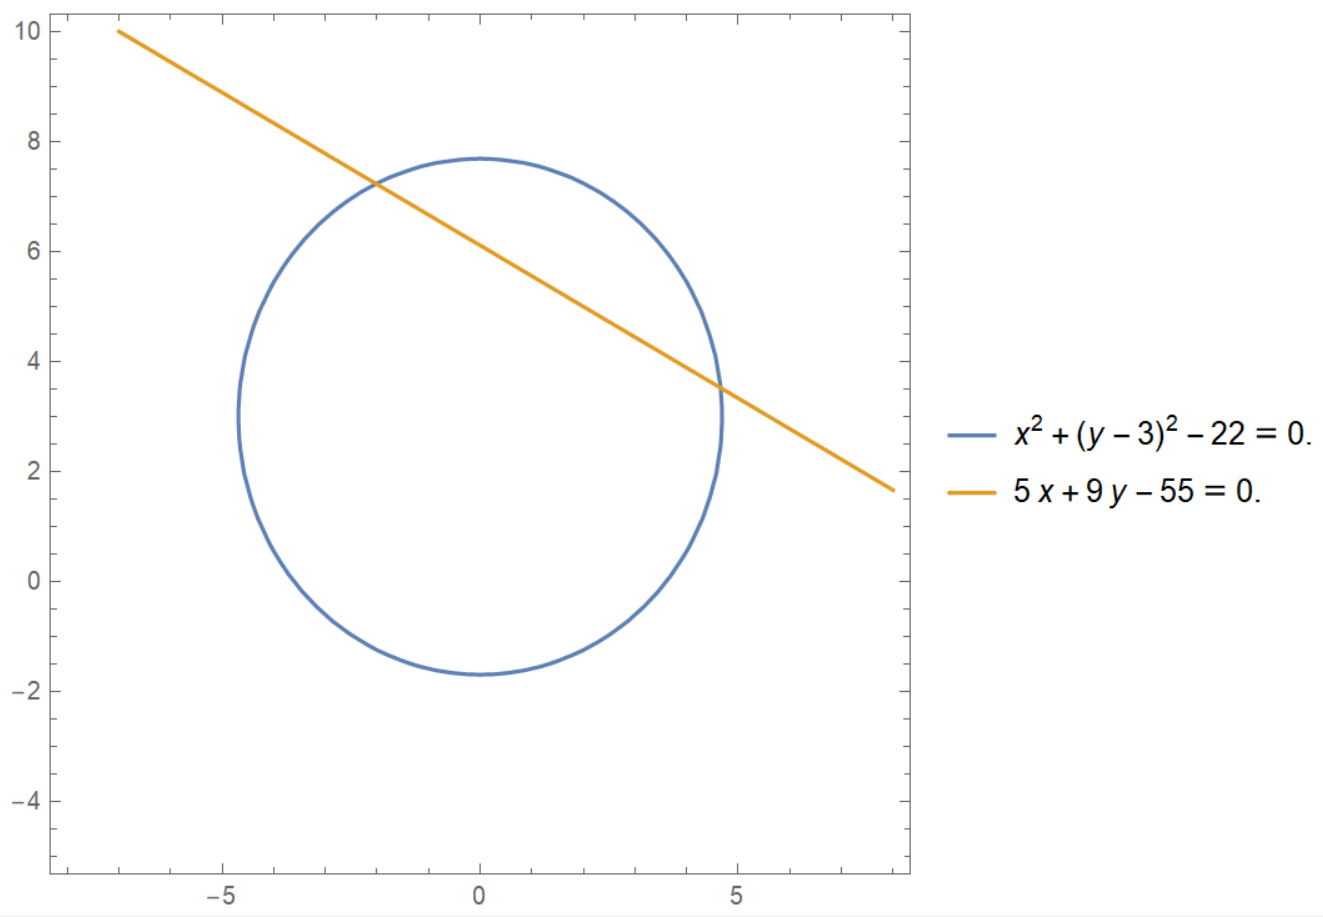
\includegraphics[scale=0.4]{pelota2}
\caption{Grafica de las posiciones balón-linea de Campo}
\label{fig:graficafun}
\end{figure}




\section{Algoritmo- Método de Newton}


i) Definir librerías\\ 

ii) Inicializar $f(x,y)$,el jacobiano $J$, semilla inicial $(x_{0},y_{0})$, la tolerancia y el numero de iteraciones máximo $n$.\\
 
iii) Repetir $k=1:n$\\

\hspace{1cm} iv) Si $\left \| f(x_{0},y_{0}) \right \|^2<tol \Rightarrow$ la raiz aproximada es $(x_{0},y_{0})$ \\

\hspace{2cm} FIN \\

\hspace{1cm} Sino Calcular: $|J(x_{0},y_{0})|$\\

\hspace{1cm} v) Si $|J(x_{0},y_{0}|=0$, imprimir ERROR, matriz jacobiana no tiene inversa. Ingresar nueva semilla\\

\hspace{1cm} vi)Sino Calcular: $(x_{1},y_{1})=(x_{0},y_{0})-(d_{1},d_{2})$ donde;\\
 
\hspace{2cm}$delta=(d_{1},d_{2})=J^{-1}(x_{0},y_{0}).f(x_{0},y_{0})$ es la variación de los $(x_{i},y_{i})$ en cada iteración \\

Nota: el calculo de la inversa del Jacobiano se hará con formula explicita(ver anexos). Para casos generales, debemos utilizar alguna algoritmo aparte que nos brinde esta.\\

\hspace{2cm} Asignar $(x_{0},y_{0})=(x_{1},y_{1})$\\

\hspace{1cm} vii)Imprimir $k,x_{0},y_{0}$\\


\section{Diagrama de flujo - Método de Newton}

\begin{figure}[h]
\centering
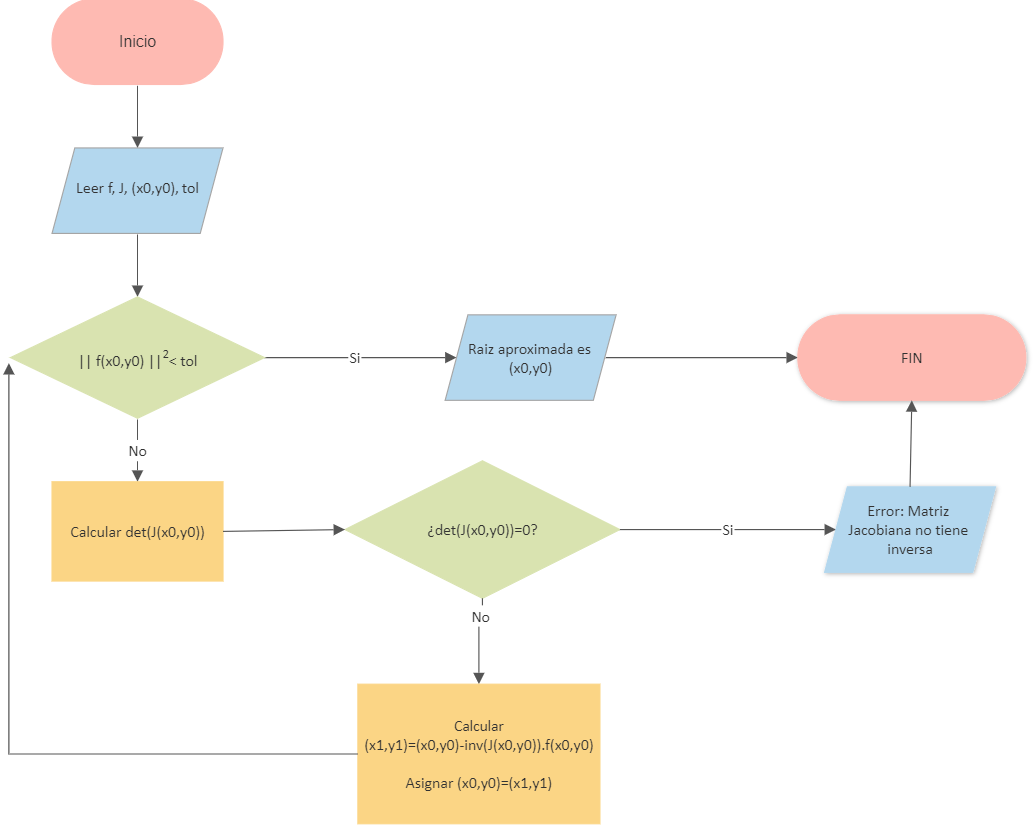
\includegraphics[scale=0.66]{flujo1}
\caption{}
\end{figure}

\section{Código C++}

\lstinputlisting{funcionf1.cpp}


\section{Resultados}

Como se observa en la Figura ~\ref{fig:graficafun} existen 2 soluciones a hallar.\\

Una primera aproximación a escoger podría ser $(x_{0},y_{0})=(0,8)$, por lo que ingresaremos a nuestro programa esta semilla, junto con un máximo de $15$ iteraciones y una tolerancia$=0.000001$. Se ve en la siguiente figura los resultados. $(x=-2.019828,y=7.233237)$

\begin{figure}[h]
\centering
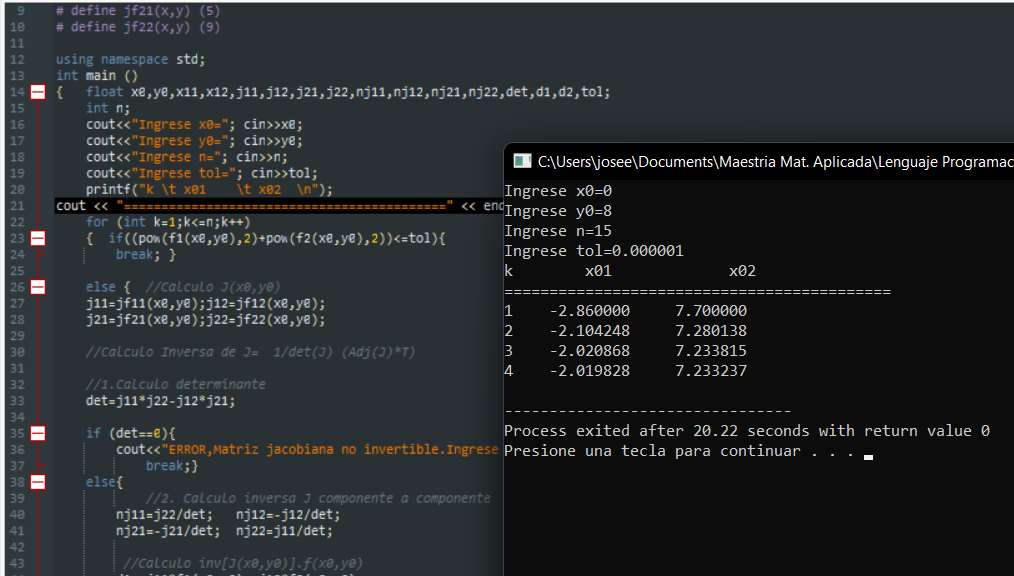
\includegraphics[scale=0.66]{resultado1}
\caption{Primer solución}
\end{figure}





Una segunda aproximación a escoger podría ser $(x_{0},y_{0})=(5,4)$, por lo que ingresaremos a nuestro programa esta otra semilla, junto con un máximo de $15$ iteraciones y una tolerancia$=0.000001$. Se ve en la siguiente figura los resultados. $(x=4.661337,y=3.521479)$

\begin{figure}[h]
\centering
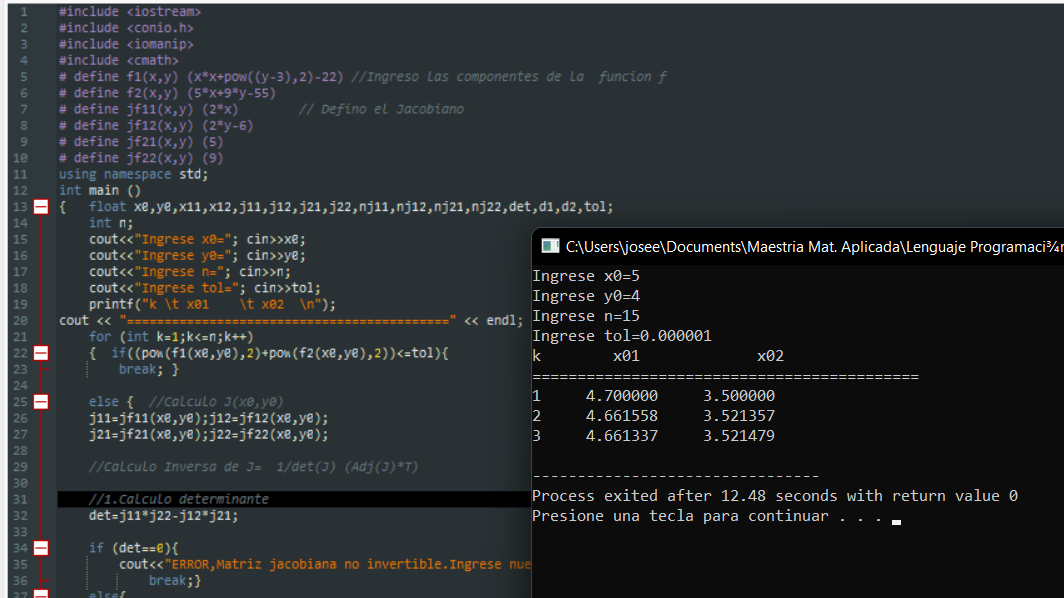
\includegraphics[scale=0.66]{resultado2}
\caption{Segunda solución}
\end{figure}


\section{ANEXOS}
En esta parte daremos las formulas explicitas de la inversa de cualquier matriz $2x2$. \\

Sea $A$ una matriz de $2x2$ cualquiera:
$$A= \begin{pmatrix}
a &b \\ 
c &d 
\end{pmatrix}$$

Esta es invertible si solo si, su determinante es distinto de cero, es decir: 
$$\left | A \right |= 
\begin{vmatrix}
a &b \\ 
c &d 
\end{vmatrix}\neq 0$$

$$ad-cb \neq 0$$

Si se cumple lo anterior, la inversa de una matriz de $2x2$ se define como: 
$$A^{-1}=\frac{1}{\left | A \right |}.\left ( Adj(A) \right )^{T}$$

$$A^{-1}=\frac{1}{\left | A \right |}
\begin{pmatrix}
d & -b \\ 
-c & a
\end{pmatrix}$$

\begin{thebibliography}{0}
  
  \bibitem{Santana} Angelo Santana del Pino.Métodos Numéricos 3. Recuperado el 9 diciembre 2022 de https://estadistica-dma.ulpgc.es/FCC/
  
  \bibitem{Venegas} P. Venegas.Departamento de Matemática
Facultad de Ciencias Universidad del Bío-Bío, Concepción. Ecuaciones y Sistemas de Ecuaciones no Lineales. Recuperado el 9 diciembre 2022 de http://ciencias.ubiobio.cl/pvenegas/220138/

    
  
\end{thebibliography}

\end{document}
